% TODO: Too much "rapid debugging" and "high-fidelity"

\section{Simple Simulator}
\label{sec:simple-simulator}
The simple simulator was developed to enable rapid testing and debugging of robot swarm behavior in a controlled 2D environment. It simulates multiple robots operating in a discretized world, rendering them as circles with their respective IDs displayed at their centers. The simulator advances in discrete time steps at 60 updates per simulated second and executes in a multi-threaded fashion to maintain performance across large robot groups. \\

The simulator supports loading map layouts from ROS 2-compatible \texttt{.pgm} files, allowing it to closely mirror environments used in the 3D Gazebo simulations. This compatibility facilitates seamless testing of behaviors across both simulation platforms. \\

\Cref{fig:simple-sim-interface} shows the graphical user interface of the simulator, displaying a scenario where three robots are performing a coordinated search in the left region of the map.

\begin{figure}[H]
    \begin{center}
        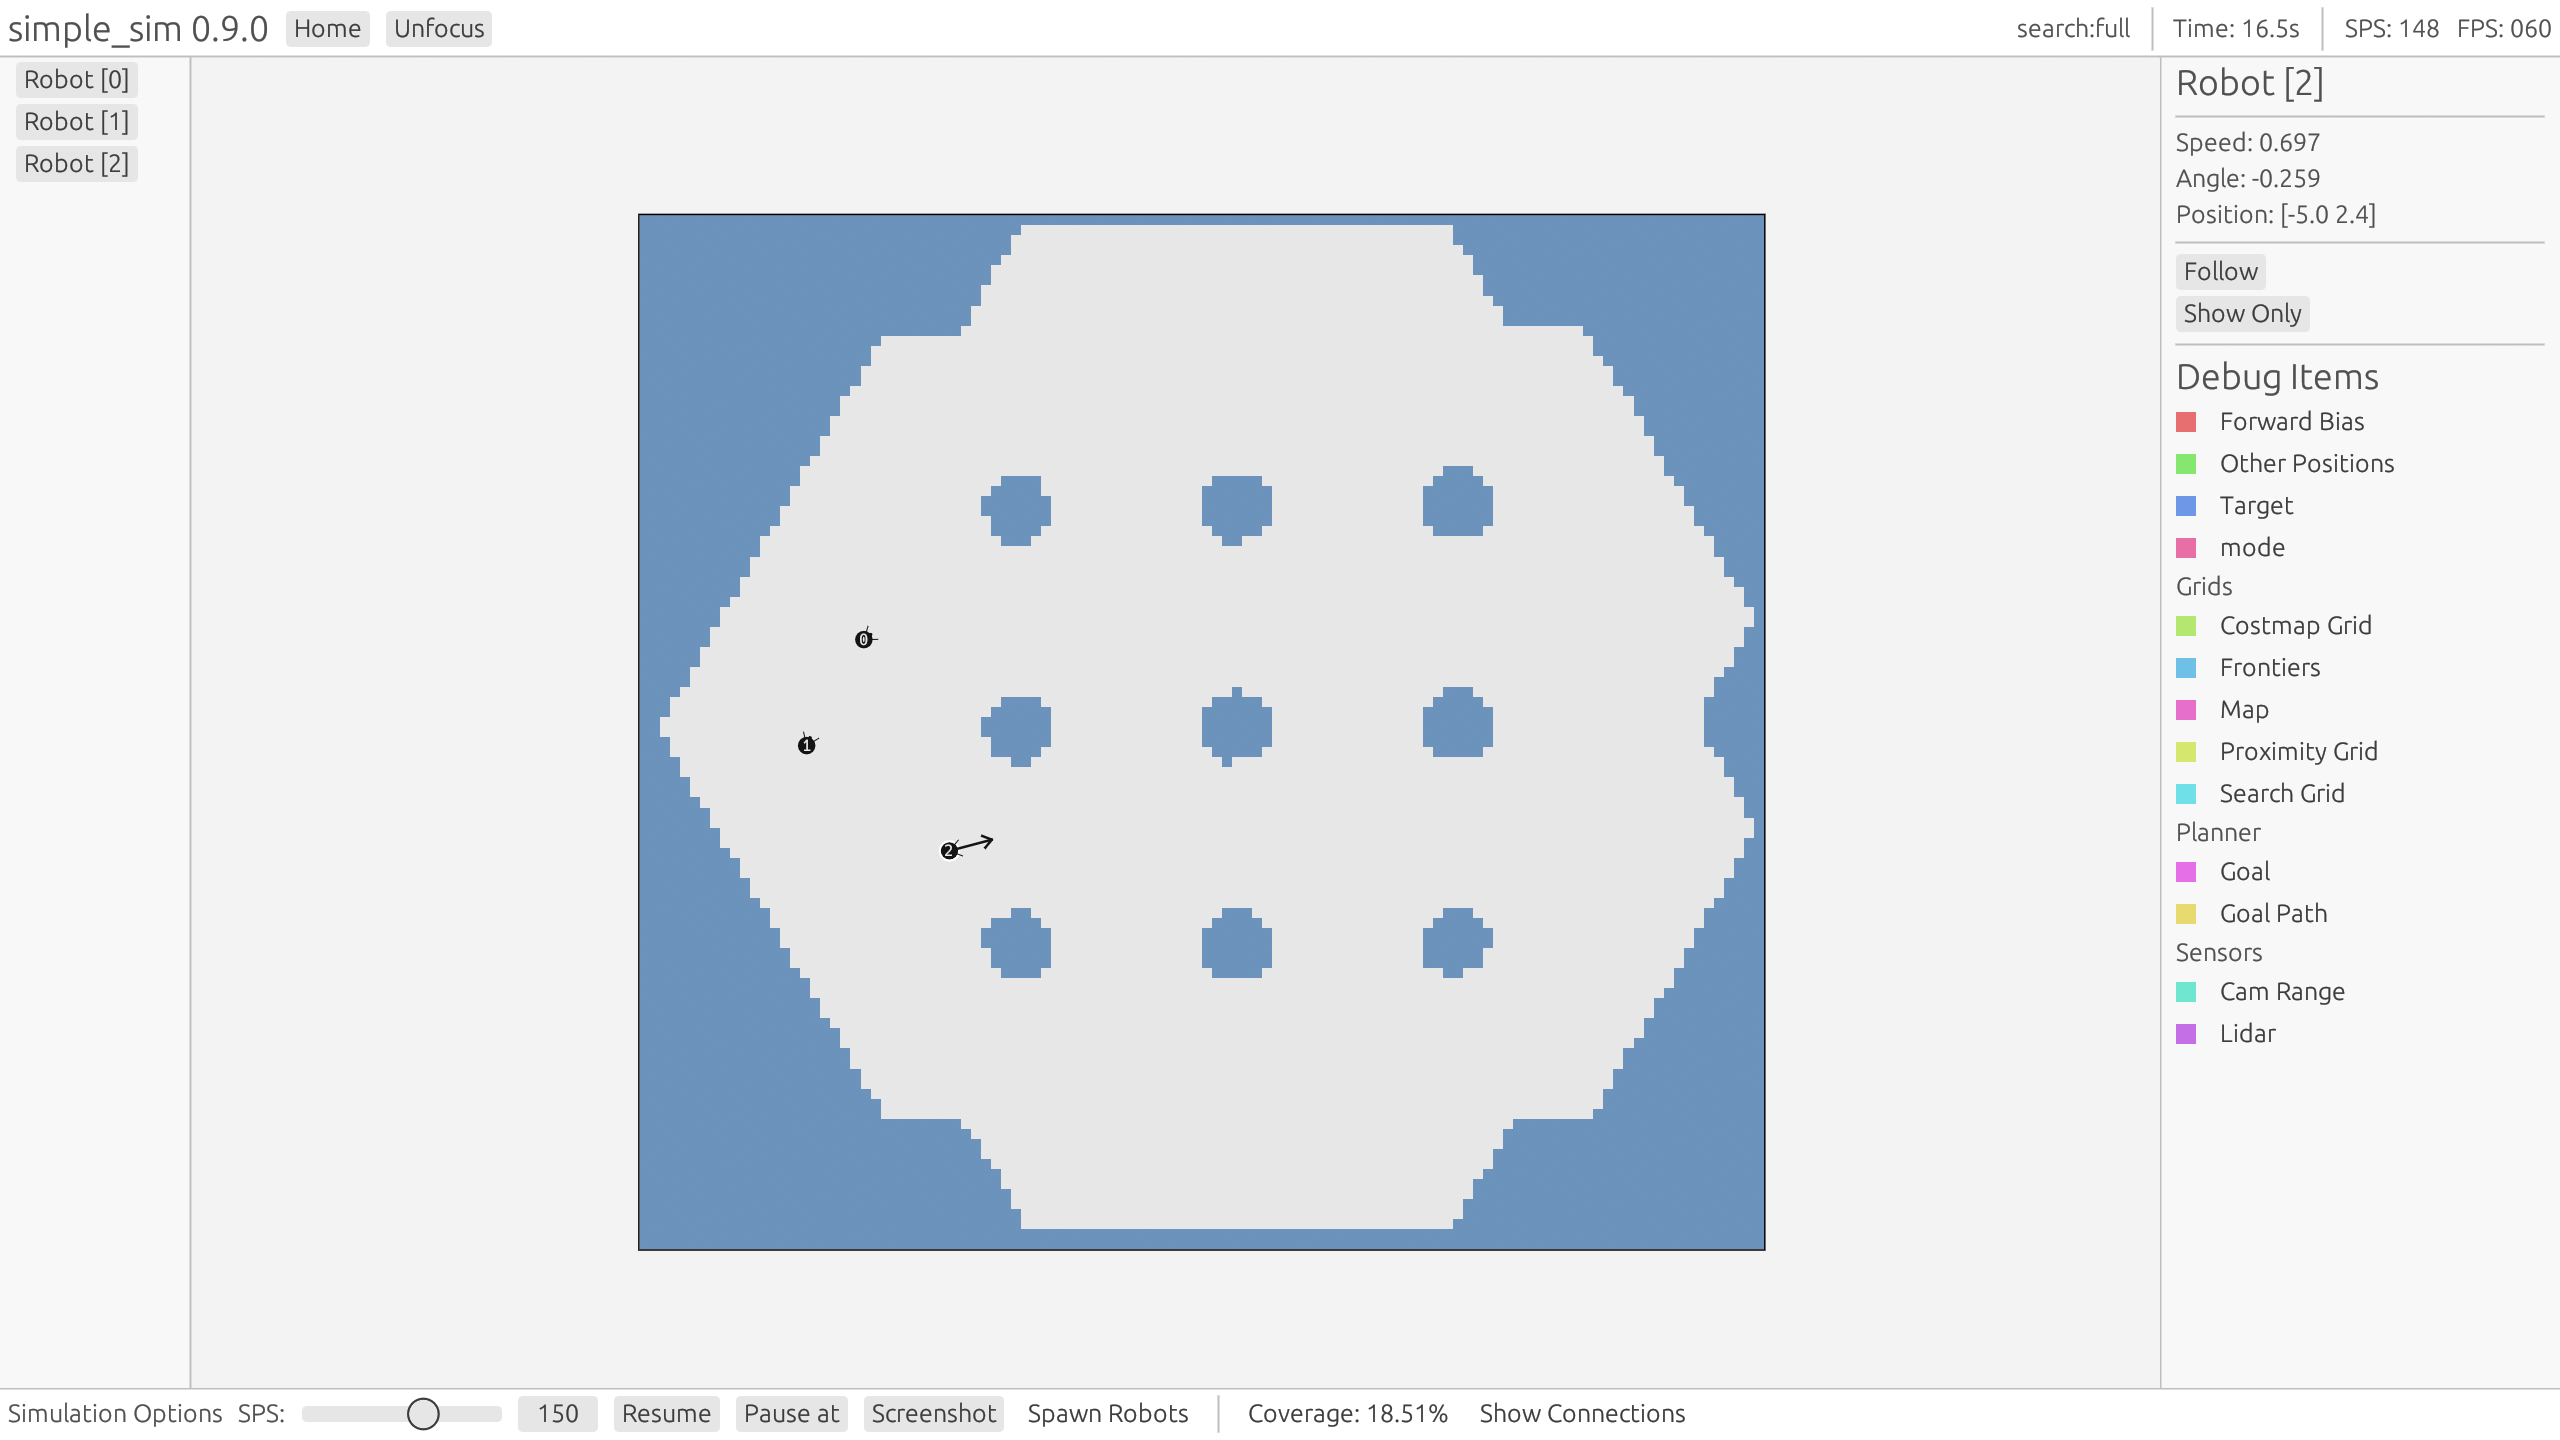
\includegraphics[width=0.95\textwidth]{figures/screenshots/simple-sim-gui.png}
    \end{center}
    \caption{Simple simulator interface showing three robots operating in a shared environment.}
    \label{fig:simple-sim-interface}
\end{figure}

\subsection{Sensor Approximation}
To run behaviors, each robot requires three inputs: pose, LiDAR, and camera data. The pose is set directly by the simulator and requires no approximation. Both LiDAR and camera inputs are emulated using simplified ray casting techniques with a constant step size. \\

LiDAR is emulated by emitting a series of radial rays from the robot's position at fixed angular intervals. Each ray is advanced incrementally until it intersects with an obstacle in the environment. The resulting distance data mimics real-world LiDAR output and is illustrated in \cref{fig:lidar-approximation}. \\

The camera emulation follows a similar ray-casting procedure, but is constrained to a defined field of view, replicating the properties of the Turtlebot 4’s camera, see \cref{fig:camera-approximation}. Rather than applying a full object detection algorithm, the camera rays directly infer object identity upon intersection, allowing simplified yet functional input for the behavior algorithms.

\begin{figure}[H]
    \centering
    \begin{subfigure}[b]{0.45\textwidth}
        \centering
        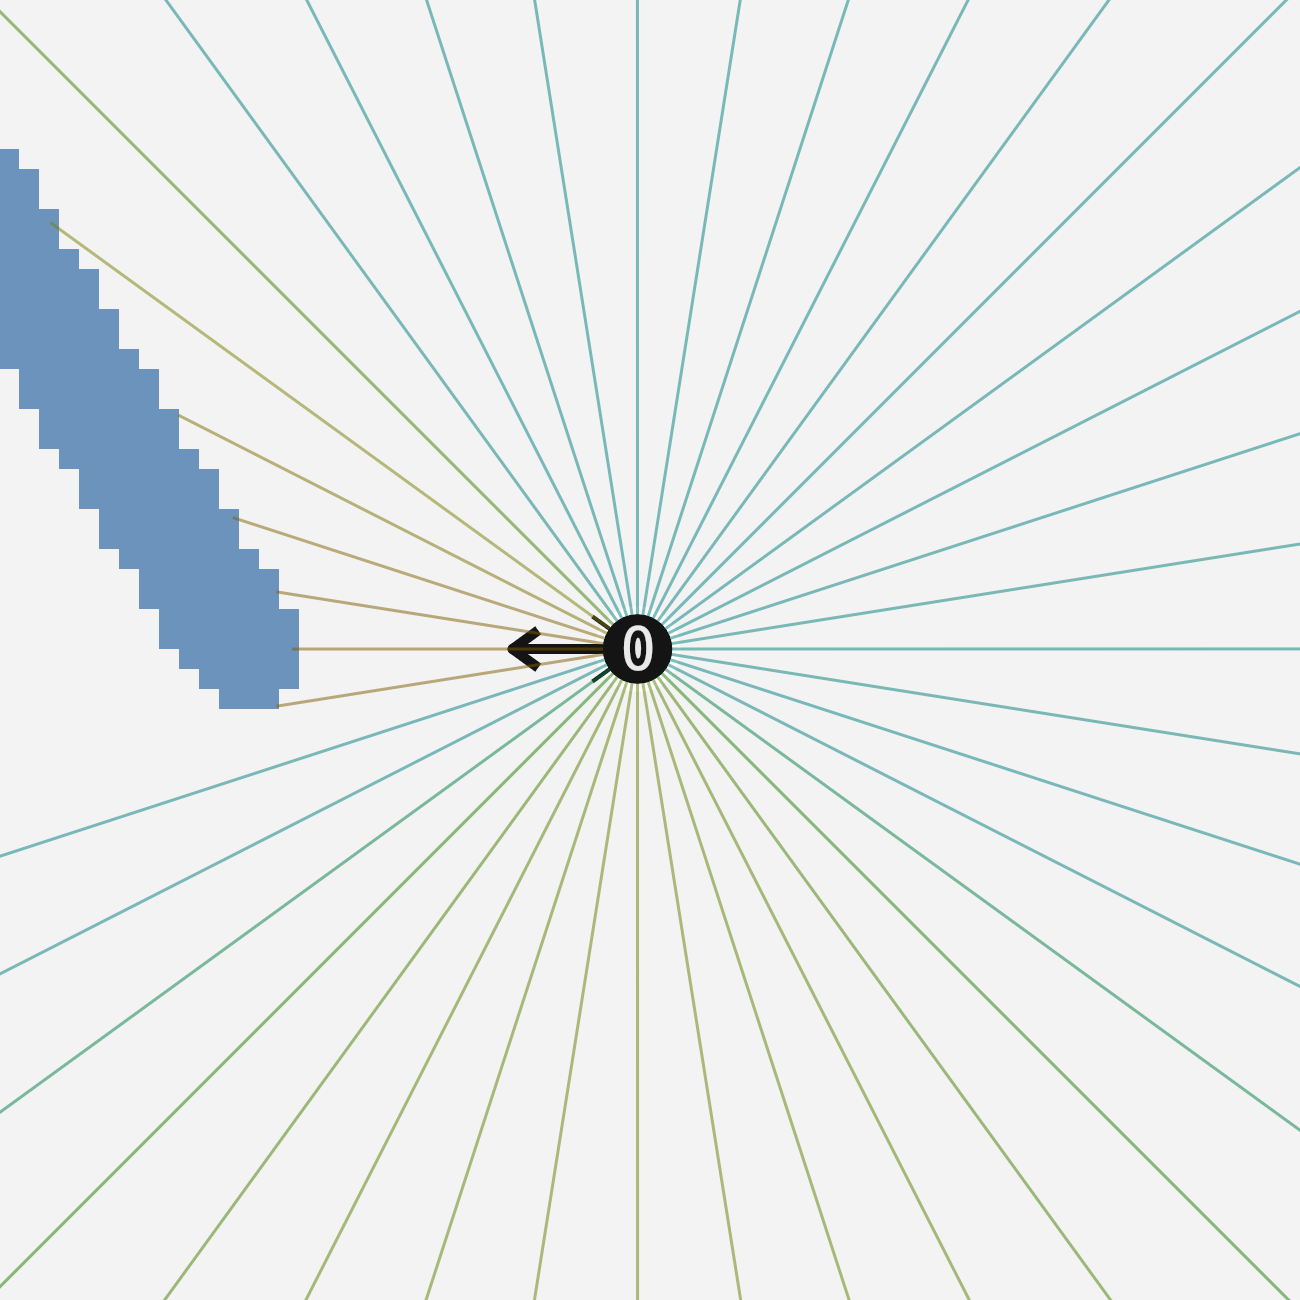
\includegraphics[width=\textwidth]{figures/screenshots/simple-lidar.png}
        \caption{LiDAR approximation.}
        \label{fig:lidar-approximation}
    \end{subfigure}
    \hfill
    \begin{subfigure}[b]{0.45\textwidth}
        \centering
        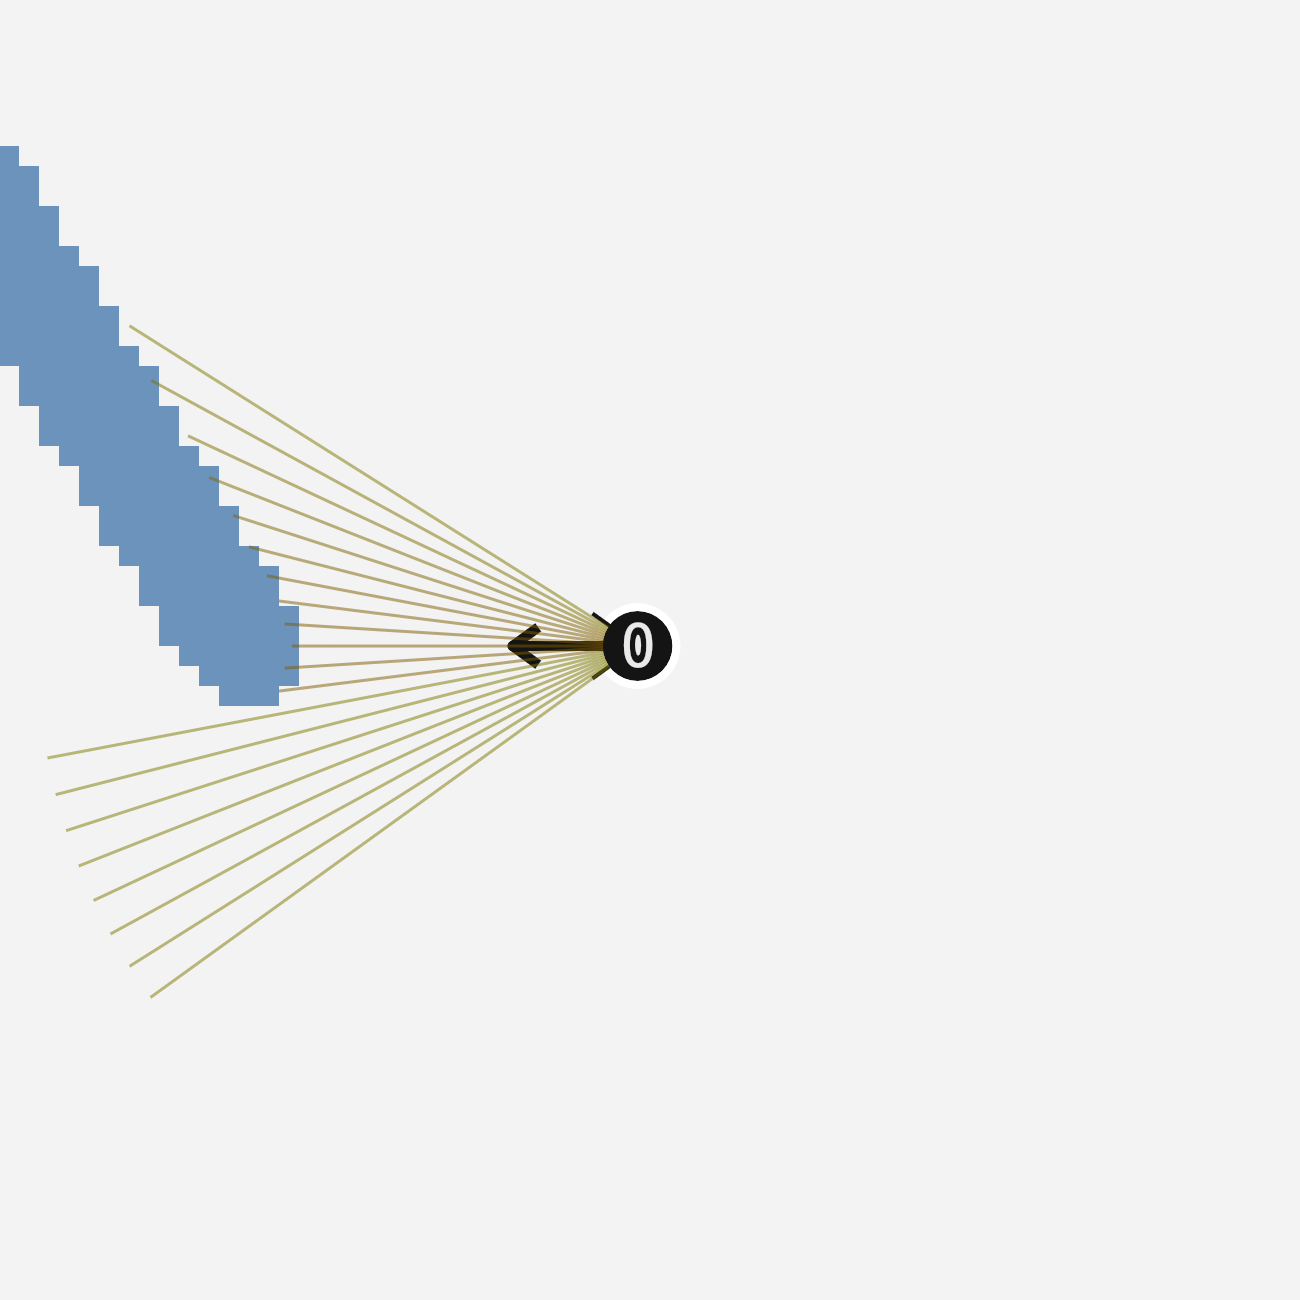
\includegraphics[width=\textwidth]{figures/screenshots/simple-camera.png}
        \caption{Camera approximation.}
        \label{fig:camera-approximation}
    \end{subfigure}
    \caption{Sensor input approximation in the simple simulator.}
    \label{fig:sensor-approximation}
\end{figure}

\subsection{\texttt{simple\_sim} as a Library}
As well as being an executable, the \texttt{simple\_sim} simulator is also implemented as a reusable library. In addition to running with a graphical user interface, it can be executed in headless mode, without visualization. This is particularly useful when running reinforcement learning experiments as explored in \cref{sec:rl}.

% Move under big section "Simple Simulator"
\subsection{Performance} 
The simple simulator is designed to be lightweight and performant. It supports deterministic execution, enabling reproducible tests for debugging. Simulation speed can be accelerated beyond real time, depending on CPU capacity and the number of robots simulated. \\

% TODO: Specify CPU used
Multi-threading is used to parallelize sensor simulation and robot state updates, allowing the system to scale to larger swarms. In practical testing, the simulator is capable of 30 to 50 robots in real time on a Macbook M1 Pro {\color{red} [CITE]} depending on the behavior. Because the environment is purely 2D and avoids expensive physics calculations, the performance overhead is minimal compared to full 3D simulation.
